\documentclass{jarticle}
\usepackage{robomech}

\usepackage{mathrsfs}
\usepackage{bm}
\usepackage[dvipdfmx]{graphicx}
\usepackage{enumerate}
\usepackage{amsmath}
\usepackage{url} 

\begin{document}
\makeatletter
\title{未知障害物環境に対応するための\\モンテカルロ自己位置推定における観測範囲の選択}
{―まだ決まってない―}
{Observation Range Selection in Monte Carlo localization for Unknown Obstacle Environments}
{-Not decided yet.-}

\author{
\begin{tabular}{ll}
 ○学\hspace{1zw} 池邉龍宏(千葉工大)& 正\hspace{1zw}林原靖男\hspace{1zw} (千葉工大)\\
 \hspace{1zw}正\hspace{1zw}上田隆一(千葉工大)\\
 % ※協賛・後援団体の会員資格で発表される場合は「正・学」は不要です。
 \end{tabular}
 % &\\
 \vspace{1zh} \\
 \begin{tabular}{l}
{\small Tatsuhiro IKEBE, Chiba Institute of Technology, 
 }\\
 {\small Yasuo HAYASHIBARA, Chiba Institute of Technology}\\
 {\small Ryuichi UEDA, Chiba Institute of Technology}\\
\end{tabular}
}
\makeatother

\abstract{ \small 
Not decided yet.
}

\date{} % 日付を出力しない
\keywords{Autonomous mobile robots, Navigation, LiDAR Localization, MCL, Unknown Obstacle}

\maketitle
\thispagestyle{empty}
\pagestyle{empty}


\section{緒言}%===========================

屋外での自律移動ロボットの自己位置推定は、
Monte Carlo localization(MCL)\cite{gutmann2002}と、
LiDARの組み合わせで行われることが多い。
MCLは確率的な自己位置推定手法で、
センサの情報をベイズの定理で位置の情報に変換する。
具体的には、数百程度のロボットの位置と向きの候補(パーティクル)を
データとして持ち、センサの情報と一致するパーティクルを残していくことで、
尤もらしい位置と向きを求める。
LiDAR(Light Detection and Ranging)は
2次元あるいは3次元のレーザースキャナのことを指し、
ロボットから壁などの障害物までの距離を、
1点ではなく平面状、あるいは立体的に計測できる。


この組み合わせの場合、
ロボットにはLiDARのセンシング対象となる、
壁などの障害物の位置を記録した地図を持たせることになる。
MCLはLiDARからの距離の情報と地図の障害物の位置を
比較し、ロボットの位置と向き(位置と向きをあわせて、以後「姿勢」と呼ぶ)を求める。


この方式の場合、地図に記載のない障害物が雑音となる。
屋外では歩行者や走行中、停車中の自動車、自転車などが、
地図に記載できない障害物となる。
例として、図\ref{fig:つくばチャレンジ人混み}に、
つくばチャレンジ\cite{つくばチャレンジ}の様子を示す。
つくばチャレンジというのは、
実際に人や自動車が通る横断歩道、公園において、
ロボットを約2[km]自律走行させる技術チャレンジである。
図\ref{fig:つくばチャレンジ人混み}を撮影したときは、
ロボットを見物する人がスタート地点に押し寄せており、
LiDARの示す障害物と地図上の障害物が一致しない状況であった。
特に2次元のLiDARを用いる場合、このような状況に対し、
MCLの側でなんらかの対策をしないと、位置推定が破綻しやすくなる。

この問題への対策の例として、
富沢ら\cite{富沢2012}、赤井ら\cite{赤井2019}の研究事例がある。
富沢ら\cite{富沢2012}は、LiDARの値から周囲の地図を作成し、
パーティクルの姿勢ごとにロボットの持つ地図と照合して不一致度を求め、
ロボット周辺が地図と異なる状況になっていることを検知した。
一方、赤井ら\cite{赤井2019}は、ロボットの姿勢とセンサ観測のクラス
@@@これなに?@@@を同時推定する方法を提案した。
この手法により、LiDARの値が、地図上の障害物からのものかそうでないかを判別した。
%@@@↓何言ってるかわからん@@@
%これを利用し、既知障害物のみを含む観測
%センサ観測のみをパーティクルの観測更新に使用することで、
%動的障害物やランドマークの移動・除去に関する環境変化に対して、
%頑健に位置推定ができることを確認している。

%@@@↓論理展開が意味不明。何をするか具体的に書いてない。論文ではアイデアとか口語的な表現を使わない。@@@
%これらの従来研究の未知障害物を観測に含めないことで、自己位置推定の破綻を防ぐという
%考えから、パーティクルごとに観測範囲を持たせるというアイデアを得た。
%そこで、本稿では、そのアイデアをMCLに実装し、実装後のMCLの性能について評価する。

これらの手法は、移動ロボットでも有効性が検証されている一方、
計算量が通常のMCLより大きくなる。
そこで筆者らは、「地図にない障害物に当たったレーザーを無視」することを考えた。
逆に言うと、センサから送られてくる情報から、
自己位置推定に有効なものだけを選別して利用するという考え方となる。
この方法の場合、MCLへ入力されるセンサ情報は減るので、
選別アルゴリズムの計算量が小さければ、むしろ全体の計算量は減少する。

そこで本稿では、地図にない障害物に
当たったであろうレーザーを無視する簡素な手法をひとつ示し、
この手法を評価する。この評価により、
自己位置推定に有効なセンサ情報を選別する手法の可能性を議論する。
2章では、実装した地図にない障害物への対策方法、
3章では実験の方法を説明する。
4章では実験結果について議論し、5章で本稿をまとめる。

\begin{figure}[bth]
  \centering
	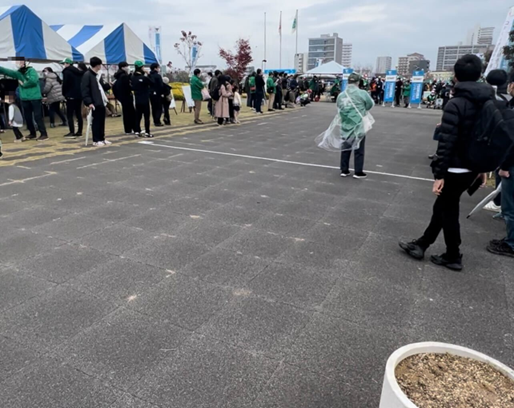
\includegraphics[width=0.8\linewidth]{fig/hitogomi.png}
   \caption{Crowds at the starting point of Tsukuba Challenge 2022}
   \label{fig:つくばチャレンジ人混み}
 \end{figure}

\section{観測範囲を制限したMCL}%===========================

実装する手法は、ひとつのパーティクルが
使うLiDARの観測範囲を制限し、
パーティクルごとに観測範囲を変えるというものである。
たとえば2次元LiDARで、ロボット前方を$0$[deg]としたときに
左右$\pm \varphi_\text{max}$[deg]の範囲が計測できるとする。
このとき、MCLで各パーティクルの重みを変えるとき、
$\varphi^{(i)} \pm \Delta\varphi^{(i)}$[deg]
の範囲の距離計測値しか用いない。
ここで$i$は$i$番目のパーティクルという意味である。
つまり、パーティクルによって距離計測値の範囲を変える。
また、$ -\varphi_\text{max} \le -\Delta\varphi^{(i)}$、
$\Delta\varphi^{(i)} \le \varphi_\text{max}$とする。

このように観測範囲を限定する狙いは、
地図にない障害物に観測範囲が向いている
パーティクルを減らすことである。
たとえば自己位置推定が安定している状態で
ロボットが直線状の通路を全身してり、
右の路肩に地図には記載のない乗用車が
停車している状況を考える。
このとき、パーティクルのうち、
観測範囲が乗用車に向いているものは、
地図とLiDARからの値の整合性がとれず、
リサンプリングの際に消去されやすい。
この際、生き残ったパーティクルは、
複製される。
このような淘汰が進むと、
パーティクルが地図に記載されていない
障害物の観測を避けるようになる。


また、1割程度の各パーティクルに対してランダムな観測範囲を再付与させる。

\section{実験}%===========================

\subsection{実験環境}

2章で説明した手法を実装し、その効果の検証をするためにシミュレータ環境を用いた。
今回、使用した環境を図\ref{fig:人混みガゼボ}、
\ref{fig:つくばチャレンジ人混みシミュレータ}に示す。
この環境は、図\ref{fig:つくばチャレンジ人混み}のつくばチャレンジでの人混みの環境を模したものである。
環境には、人型や箱型の未知障害物を多く配置した。全ての未知障害物は速度0[m/s]である。

今回使用したPCの環境を表\ref{table:PCの環境}に示す。
シミュレータのソフトウェアとしてGazebo、ナビゲーションのシステムとしてROS Noeticを使用する。

実験に用いるシミュレータ内のロボットは、図\ref{fig:raspicat}のような差動二輪型のロボットである。
ロボットおよび搭載しているセンサの性能について、表\ref{table:ロボットおよび搭載しているセンサの性能}に示す。
図\ref{fig:raspicat}には示されていないが、1[m]の高さに観測用のセンサとして、2D LiDARを搭載している。
2D LiDARの観測範囲は360[deg]であり、角度分解能は1[deg]である。
ロボットの最高速度は、3[m/s]である。

\begin{table}[hbtp]
  \caption{experimental environment}
  \label{table:PCの環境}
  \centering
  \begin{tabular}{lcr}
    \hline
    CPU & Core™ i9-12900K × 24 \\
    GPU & GeForce RTX 2060 \\
    Ubuntu & 20.04 \\
    ROS  & Noetic \\
    Gazebo  &  9.0 \\
    \hline
  \end{tabular}
\end{table}

\begin{table}[hbtp]
  \caption{performance of the robot and on-board sensors}
  \label{table:ロボットおよび搭載しているセンサの性能}
  \centering
  \begin{tabular}{lcr}
    \hline
    ロボットの最高速度 & 3[m/s] \\
    2D LiDARの取り付け高さ & 1[m] \\
    2D LiDARの観測範囲 & 360[deg] \\
    2D LiDARの角度分解能 & 1[deg] \\
    \hline
  \end{tabular}
\end{table}

\begin{figure}[htbp]
  \centering
   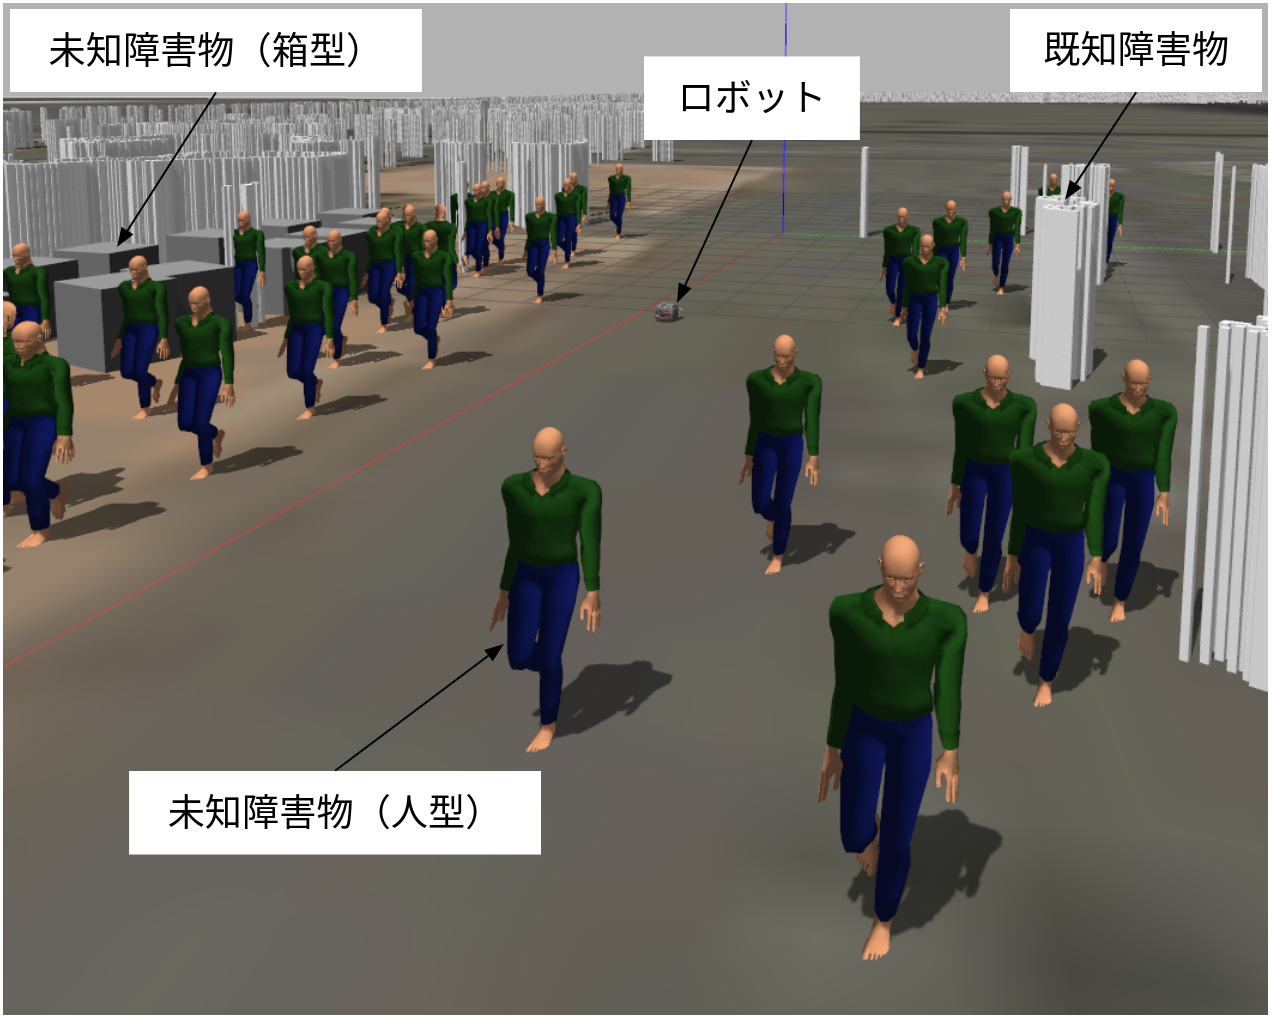
\includegraphics[width=0.8\linewidth]{fig/hitogomi_gazebo.png}
   \vspace*{-4mm}
   \caption{A simulator that mimics the crowds at the start of Tsukuba Challenge 2022}
   \label{fig:人混みガゼボ}
\end{figure}

\begin{figure}[htbp]
  \centering
   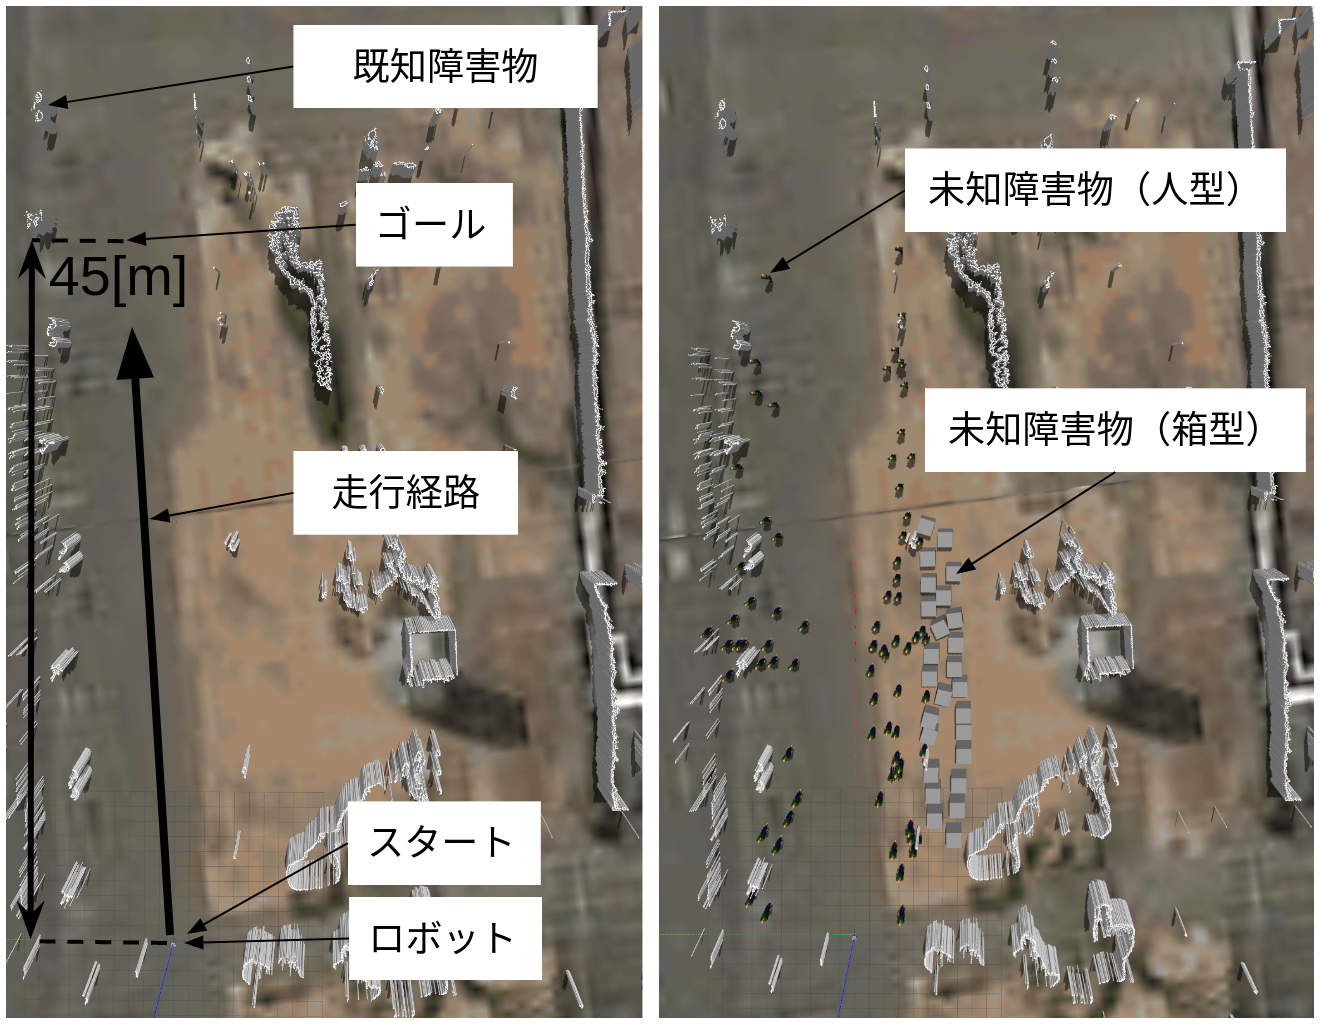
\includegraphics[width=0.8\linewidth]{fig/environment_comparison.png}
   \vspace*{-4mm}
   \caption{Environment without unknown obstacles (left), environment with unknown obstacles (right)}
   \label{fig:つくばチャレンジ人混みシミュレータ}
\end{figure}

\begin{figure}[htbp]
  \centering
   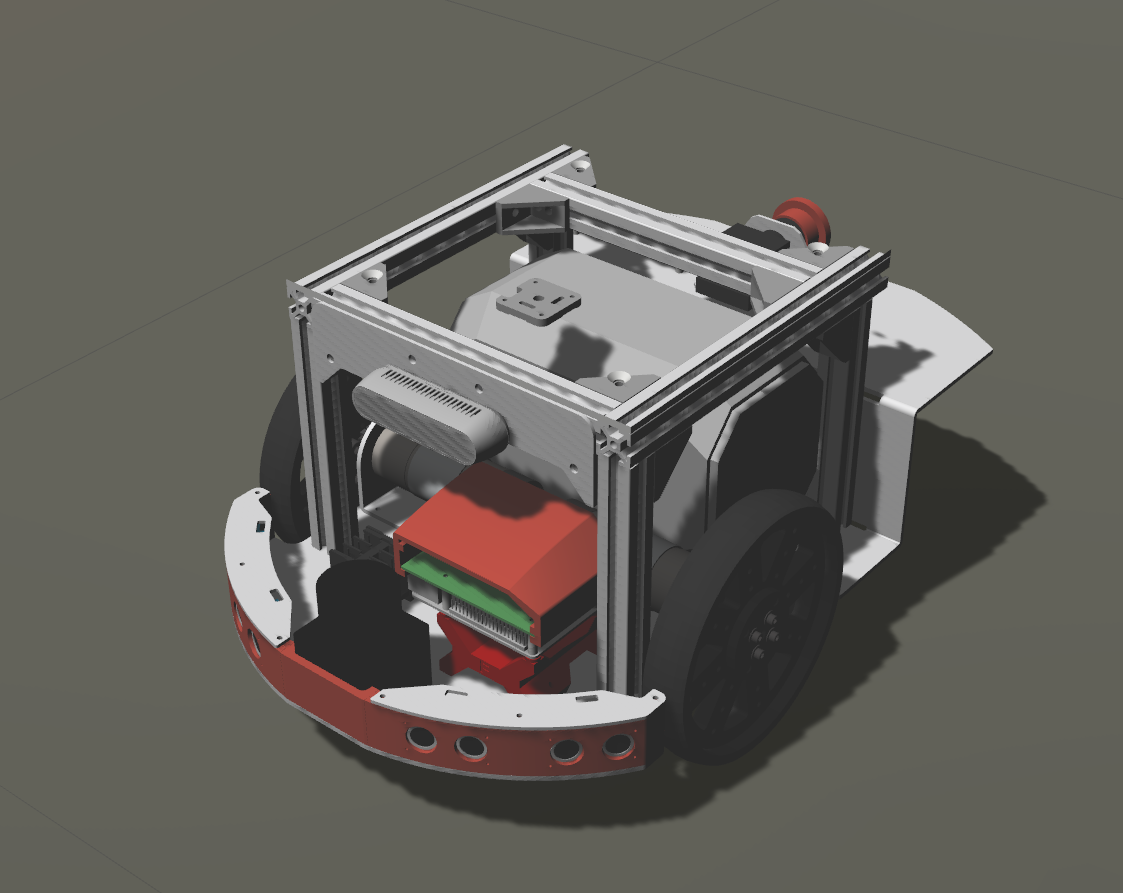
\includegraphics[width=0.8\linewidth]{fig/raspicat_gazebo.png}
   \vspace*{-4mm}
   \caption{Differential two-wheeled model robot used in the simulator}
   \label{fig:raspicat}
\end{figure}

\subsection{実験方法}

色々なパターンのパーティクルの条件で実験をする。
パーティクルの条件については、後述にて説明する。
実験方法は以下のとおりである。
\noindent
\begin{enumerate}[A]
  \item スタートからゴールまでオンラインでロボットのナビゲーションをする
  \item 事前にジョイスティックでロボットをスタートからゴールまで動かす。
        その間、得られた観測情報等を記録したデータを後から再生し、オフラインで自己位置推定をする。
\end{enumerate}
\noindent
スタートとゴールは、それぞれ図\ref{fig:スタートからゴールまでナビゲーション}
に示された位置である。

今回の実験の評価項目は、以下のとおりである。
\begin{itemize}
  \item スタートからゴールまでの100回ナビゲーションさせた場合の完走率(実験方法A)
  \item スタートからゴールまで走行したときの真値との比較(実験方法B)
  \item パーティクルの観測更新に最も使用された観測(実験方法A)
  % \item 計算時間の増減(実験方法A)
\end{itemize}

\section{実験結果}%===========================

\subsection{完走率}

表\ref{table:完走率}に、実験方法Aにより求めた、各パーティクルの条件での完走率を示す。
結果からは、観測範囲が狭くなるほど完走率が大きくなっていることがわかる。

\begin{table}[htbp]
  \caption{completion rate under certain particle conditions}
  \label{table:完走率}
  \begin{tabular}{|c|r|r|r|} \hline
  条件番号 & パーティクル数 & 観測範囲  & 完走確率 \\ \hline \hline
  \textcircled{\scriptsize 1} & 3000 & 0[deg] & 0 \\ \hline
  \textcircled{\scriptsize 2} & 3000 & 10[deg] & 0.52 \\ \hline
  \textcircled{\scriptsize 3} & 3000 & 360[deg] & 0 \\ \hline
  \textcircled{\scriptsize 4} & 10000 & 0[deg] & 0 \\ \hline
  \textcircled{\scriptsize 5} & 10000 & 1[deg] & 0.28 \\ \hline
  \textcircled{\scriptsize 6} & 10000 & 10[deg] & 0.54 \\ \hline
  \textcircled{\scriptsize 7} & 10000 & 45[deg] & 0.04 \\ \hline
  \textcircled{\scriptsize 8} & 10000 & 90[deg] & 0 \\ \hline
  \textcircled{\scriptsize 9} & 10000 & 360[deg] & 0 \\ \hline
  \textcircled{\scriptsize 10} & 10000 & 1$\sim$15[deg] & 0.54 \\ \hline
  \end{tabular}
\end{table}

各パーティクルの条件において、自己位置推定が破綻した場所を
図\ref{fig:失敗箇所}に示す。
\textcircled{\scriptsize 3}\textcircled{\scriptsize 5}\noindent
\textcircled{\scriptsize 8}\textcircled{\scriptsize 9}\noindent
の条件は、スタートから12[m]あたり、
\textcircled{\scriptsize 2}\textcircled{\scriptsize 6}\noindent
\textcircled{\scriptsize 7}\textcircled{\scriptsize 10}\noindent
の条件は、スタートから30[m]のあたりで
自己位置推定が破綻することがあった。

\begin{figure}[htbp]
  \centering
   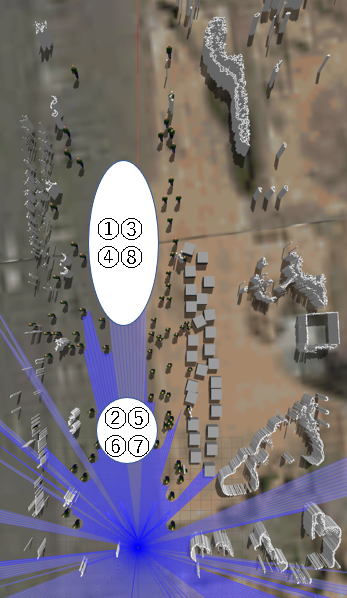
\includegraphics[width=0.8\linewidth]{fig/failure_location.png}
   \vspace*{-4mm}
   \caption{Where localization has broken down}
   \label{fig:失敗箇所}
\end{figure}

\subsection{自己位置推定の誤差}

図\ref{fig:plot}に、実験方法Bにより求めた、
真値(reference)に対する各パーティクルの条件での
自己位置推定値の誤差を示す。
まず、xy平面上に真値と自己位置推定をプロットしたものを見ると、
条件
\textcircled{\scriptsize 3}\textcircled{\scriptsize 7}\noindent
\textcircled{\scriptsize 8}\textcircled{\scriptsize 9}\noindent
の場合、スタートから約10[m]の場所から自己位置の推定誤差が大きくなり、自己位置推定破綻を起こした。
条件
\textcircled{\scriptsize 1}\textcircled{\scriptsize 4}\noindent
の場合、スタートから約19[m]の場所から自己位置の推定誤差が大きくなり、自己位置推定破綻を起こした。
条件
\textcircled{\scriptsize 2}\textcircled{\scriptsize 5}\noindent
\textcircled{\scriptsize 6}\textcircled{\scriptsize 10}\noindent
は、スタートから約15$\sim$20[m]の場所から自己位置の推定誤差が大きくなり始めたが、
20[m]以降は一定の誤差のままゴールまで到達した。
中でも条件
\textcircled{\scriptsize 5}\noindent
の誤差が小さいように見える。

xy平面上に真値と自己位置推定をプロットしたものの中でも
自己位置の推定誤差が小さかった4つの条件
\textcircled{\scriptsize 2}\textcircled{\scriptsize 5}\noindent
\textcircled{\scriptsize 6}\textcircled{\scriptsize 10}\noindent
において、真値に対する自己位置推定値のユークリッド誤差、横誤差、縦誤差
をプロットした。
4つの条件の中でも、条件
\textcircled{\scriptsize 2}\textcircled{\scriptsize 5}\noindent
の誤差が小さいように見える。
しかし、誤差が小さいといっても、それぞれの条件において、
最大で横誤差が0.4[m]、縦誤差が0.8[m]、ユークリッド誤差が0.8[m]もある。

\begin{figure}[htbp]
  \begin{center}
  \begin{tabular}{cc}
  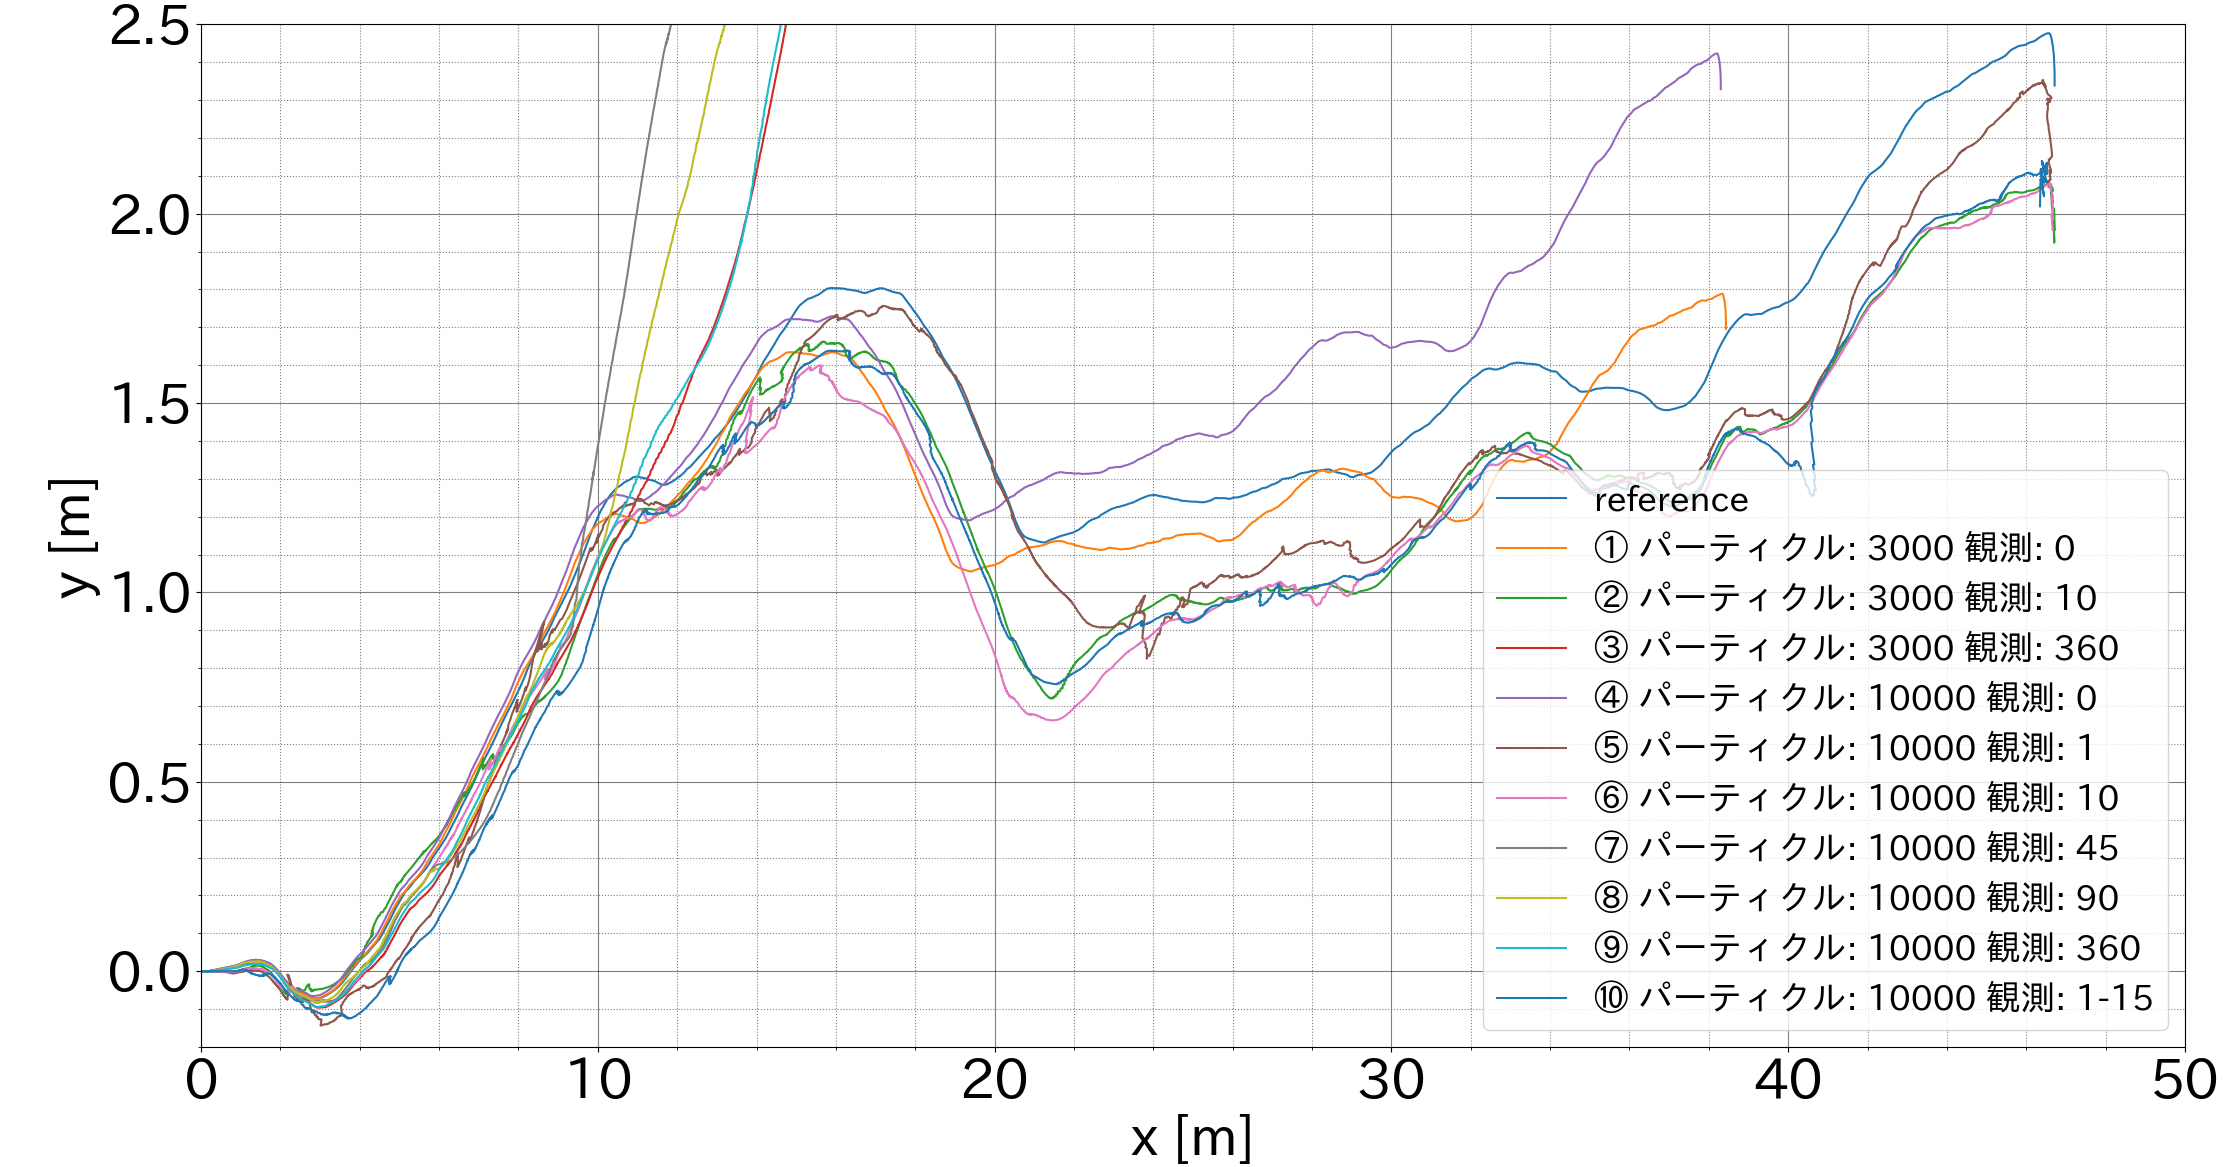
\includegraphics[width=0.8\linewidth]{fig/x_y.png} \\
  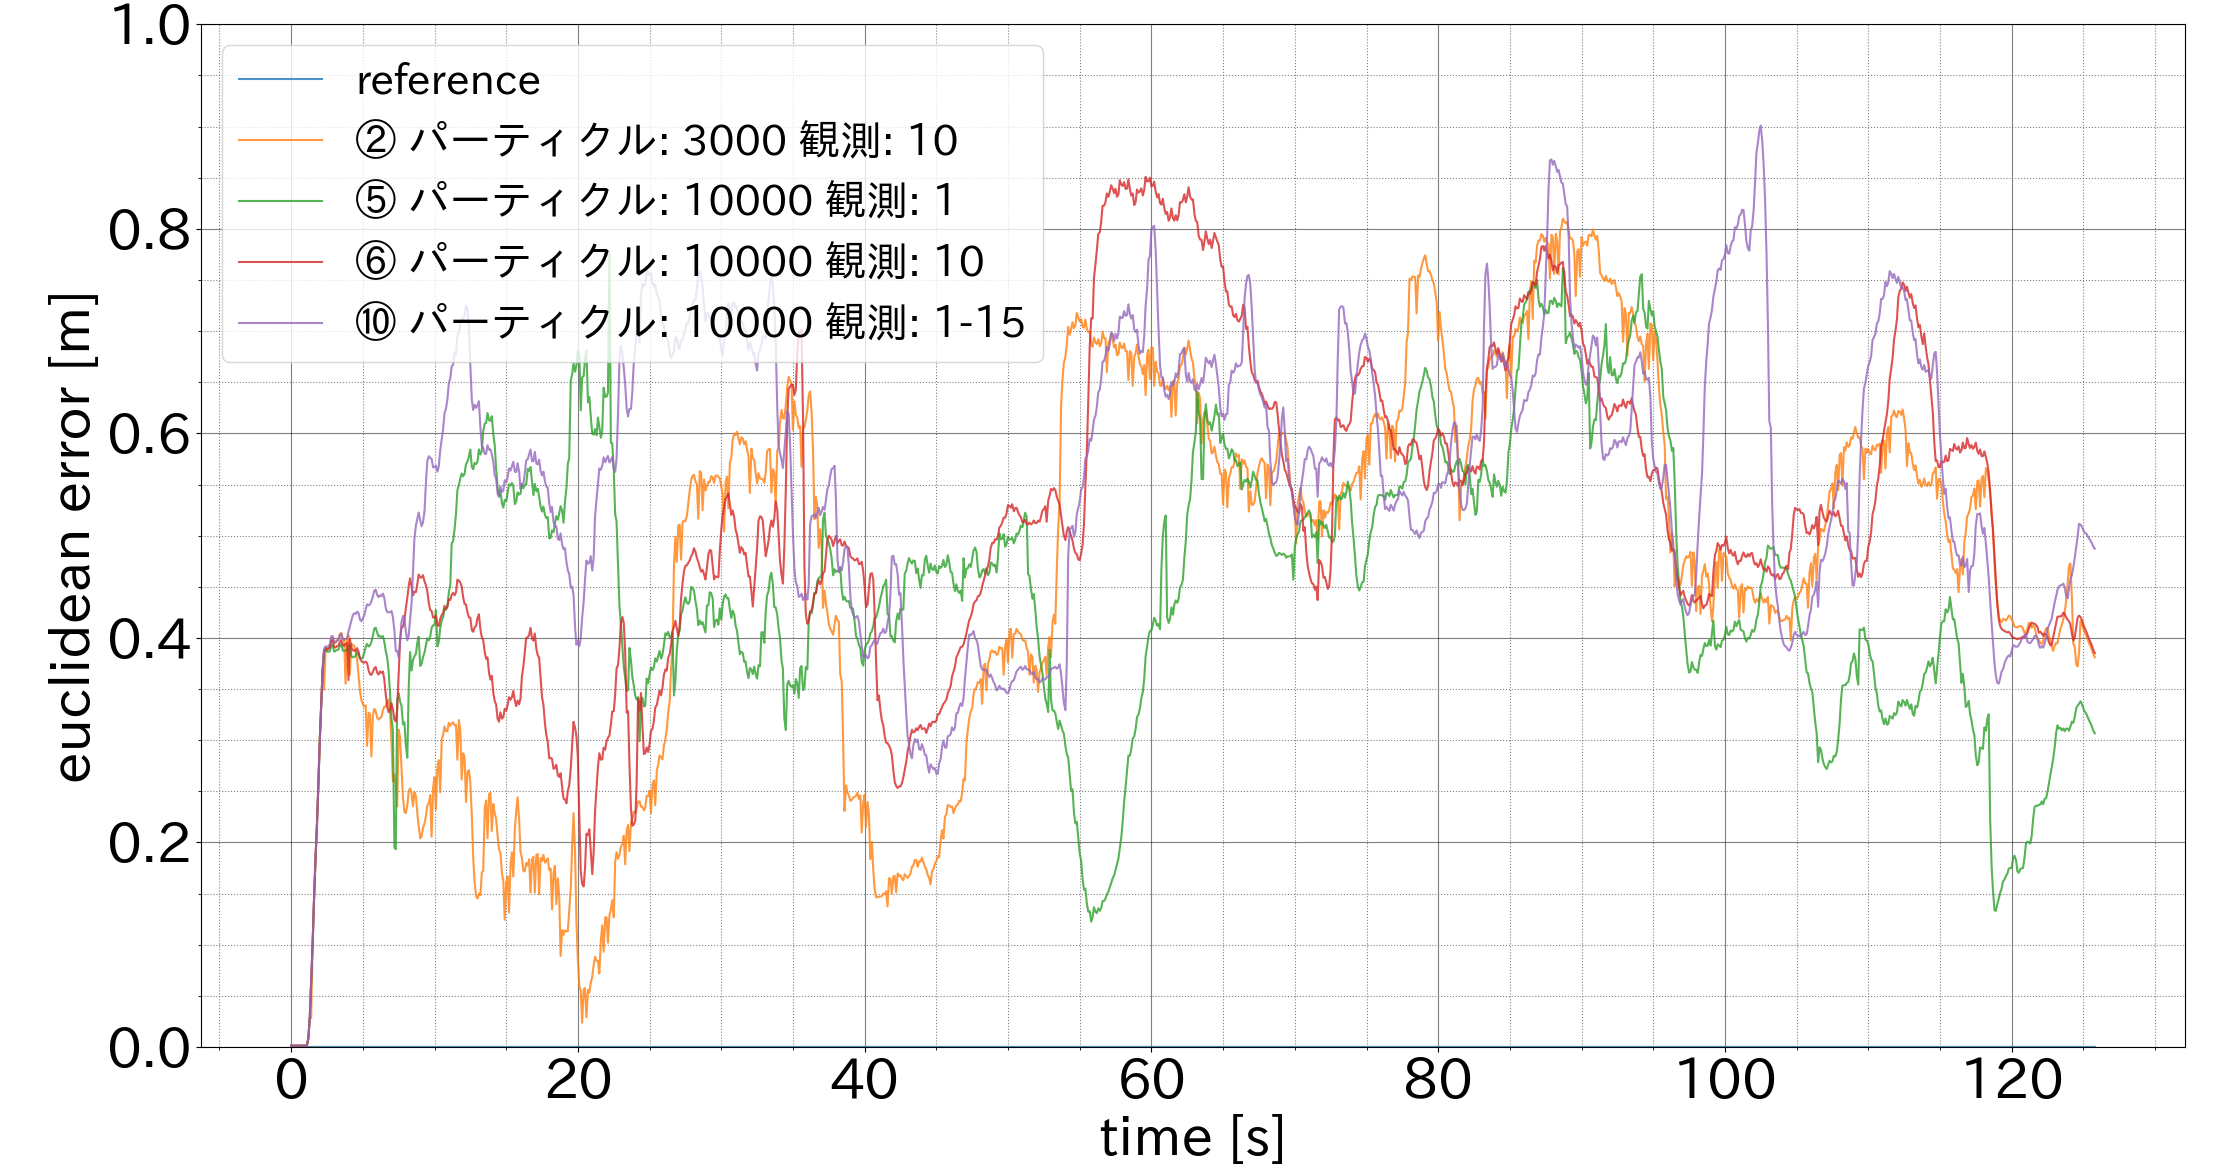
\includegraphics[width=0.8\linewidth]{fig/euclidean_error.png} \\
  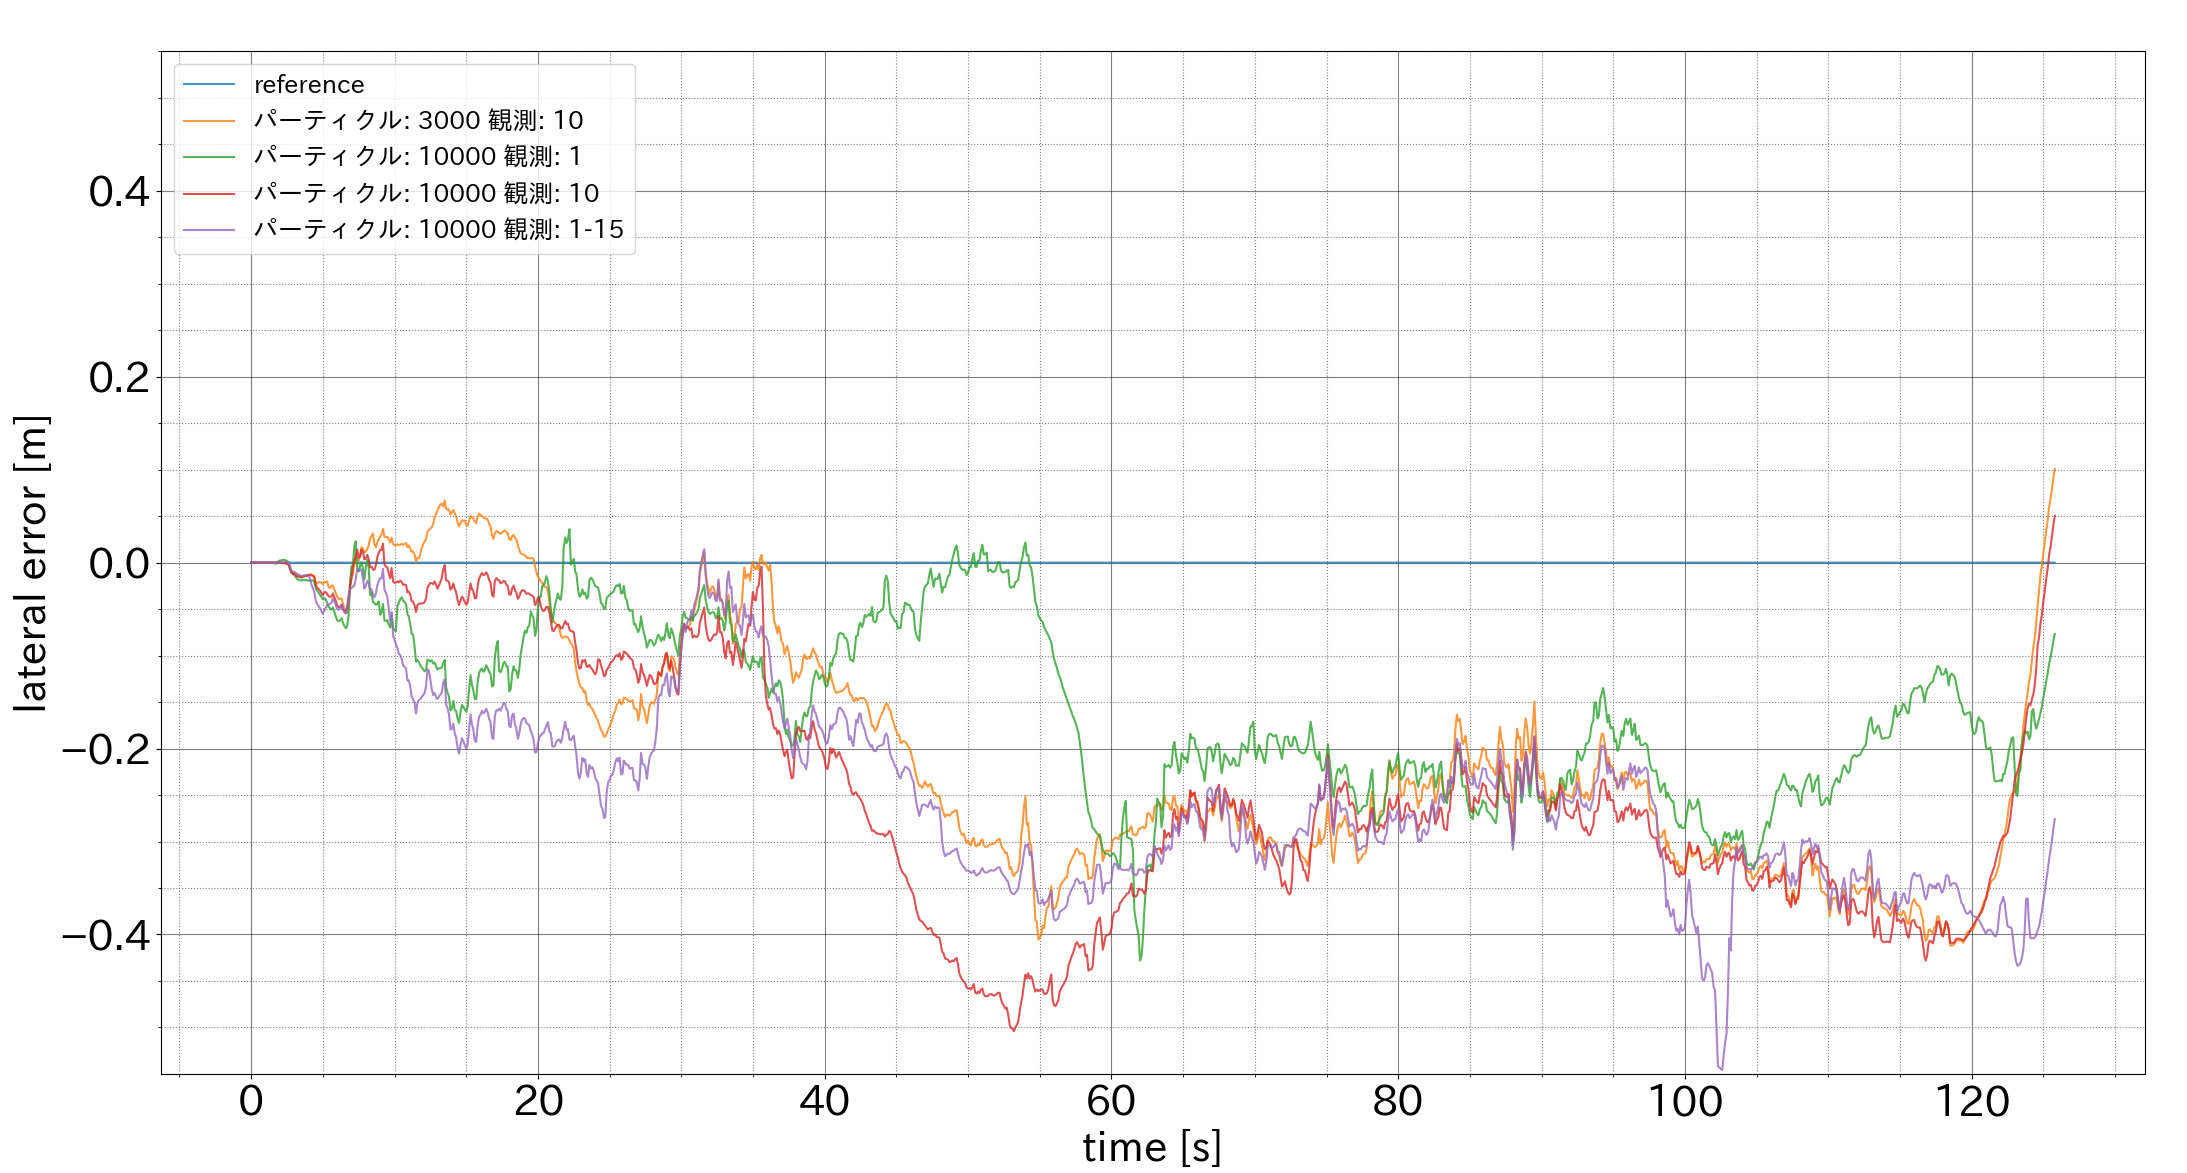
\includegraphics[width=0.8\linewidth]{fig/lateral_error.png} \\
  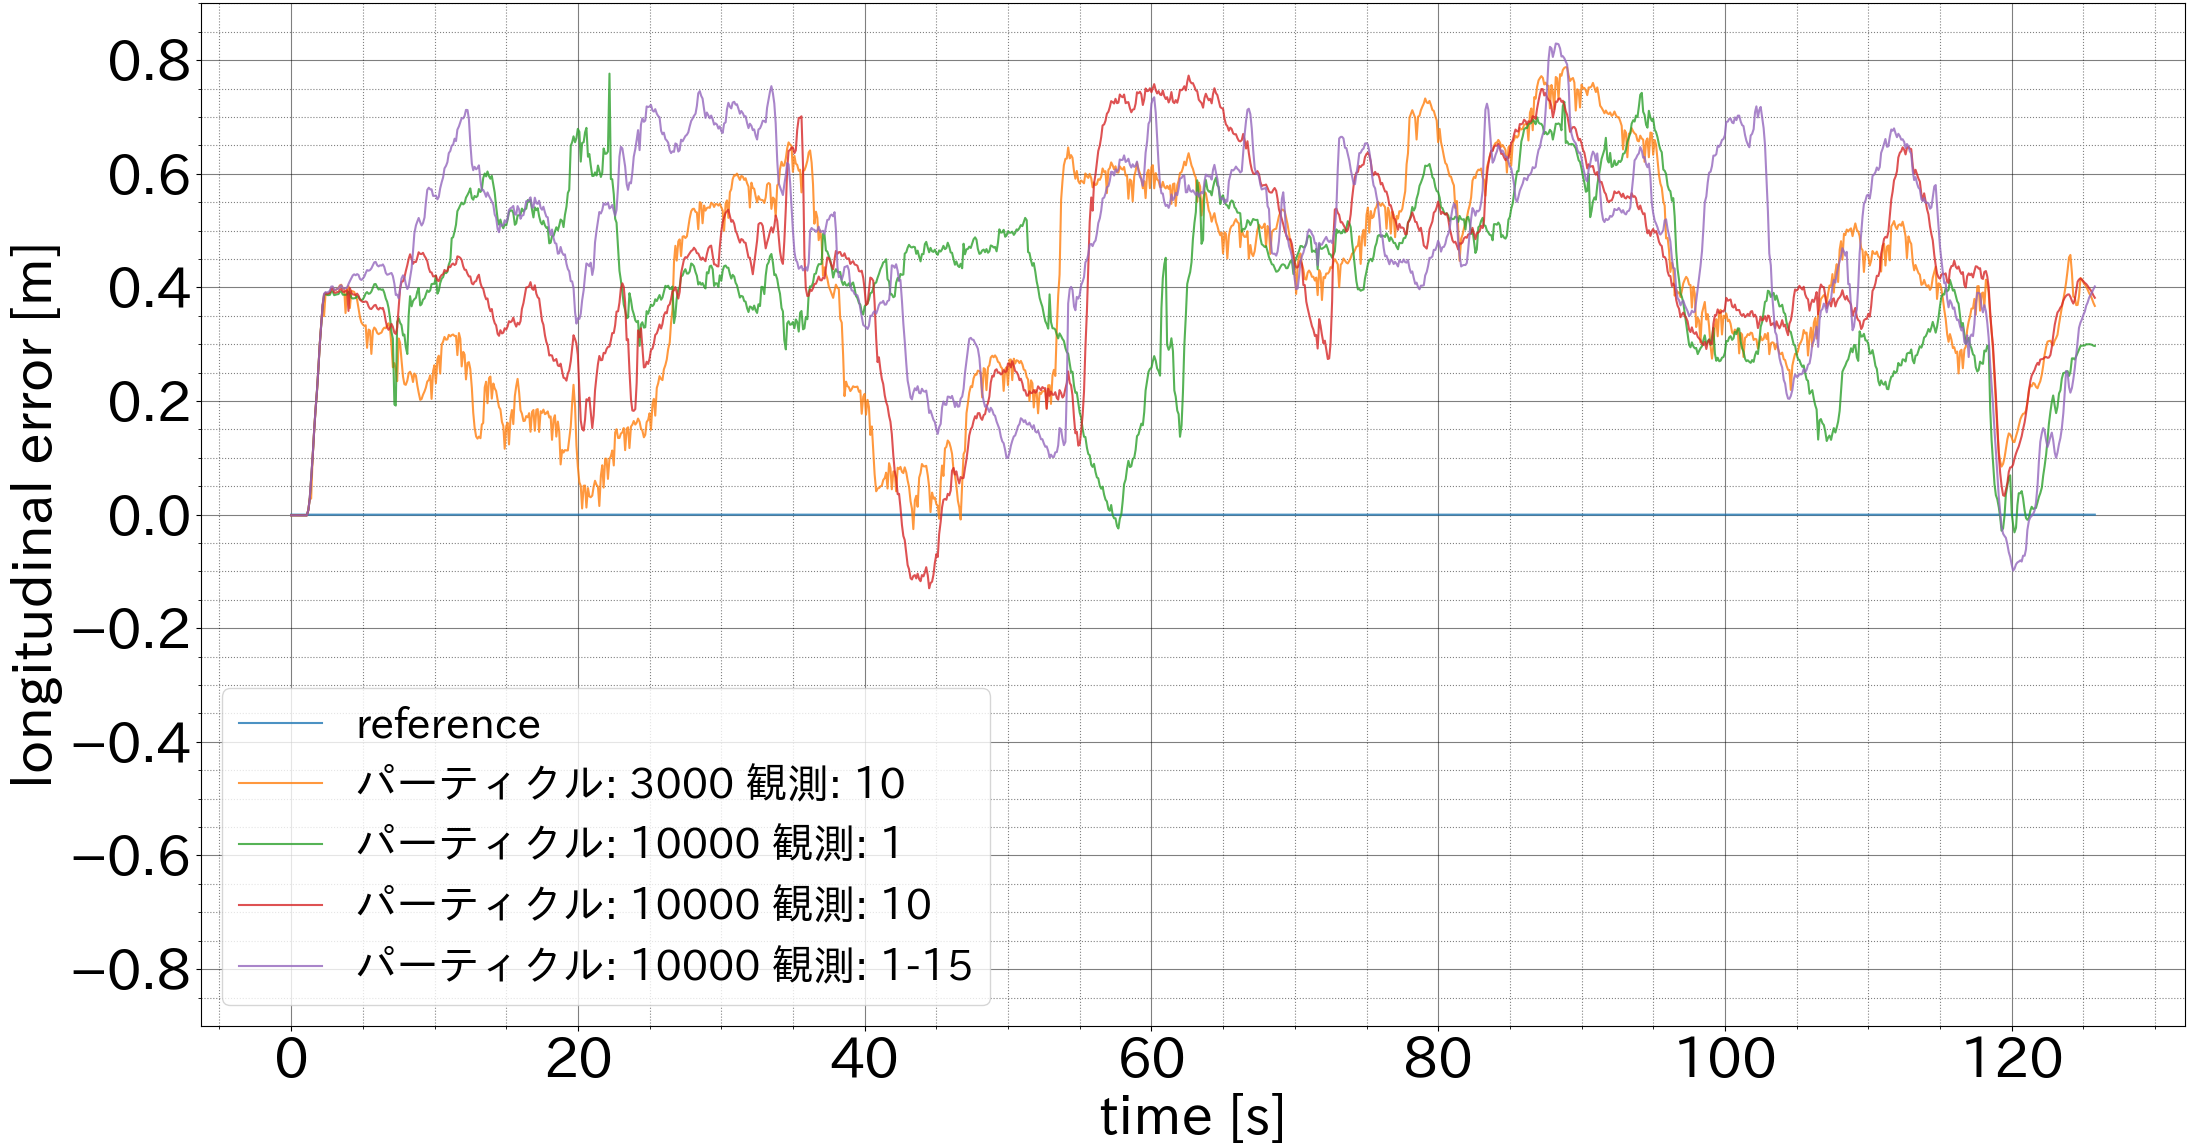
\includegraphics[width=0.8\linewidth]{fig/longitudinal_error.png} 
  \end{tabular}
  \caption{
    Plot the true value and the self-estimated position value,
     and the lateral direction and the longitudinal 
    direction and Euclidean error with respect to the true value.}
  \label{fig:plot}
  \end{center}
\end{figure}

\subsection{使用される観測}

2章で説明した手法をMCLに実装すると、
各パーティクルは観測範囲を持ち、
未知障害物が含まれないような観測を
パーティクルの観測更新に使用するようになる。
図\ref{fig:スタートからゴールまでナビゲーション}の左の図のようにロボットを
スタートからゴールまでナビゲーションをさせた時
観測更新においてどの観測を使用していたか、可視化したものを
図\ref{fig:スタートからゴールまでナビゲーション}の右の図に示す。
このときのパーティクルの条件は、パーティクルの数10000、観測範囲1[deg]である。
赤色が、スタートからゴールまでの全観測であり、
緑色が、手法の実装によって既知障害物の観測として求められた観測である。
未知障害物の観測であるのに緑色になっている部分が少しあるが、
ほとんど既知障害物の観測を選択していることがわかる。

\begin{figure}[t]
  \centering
   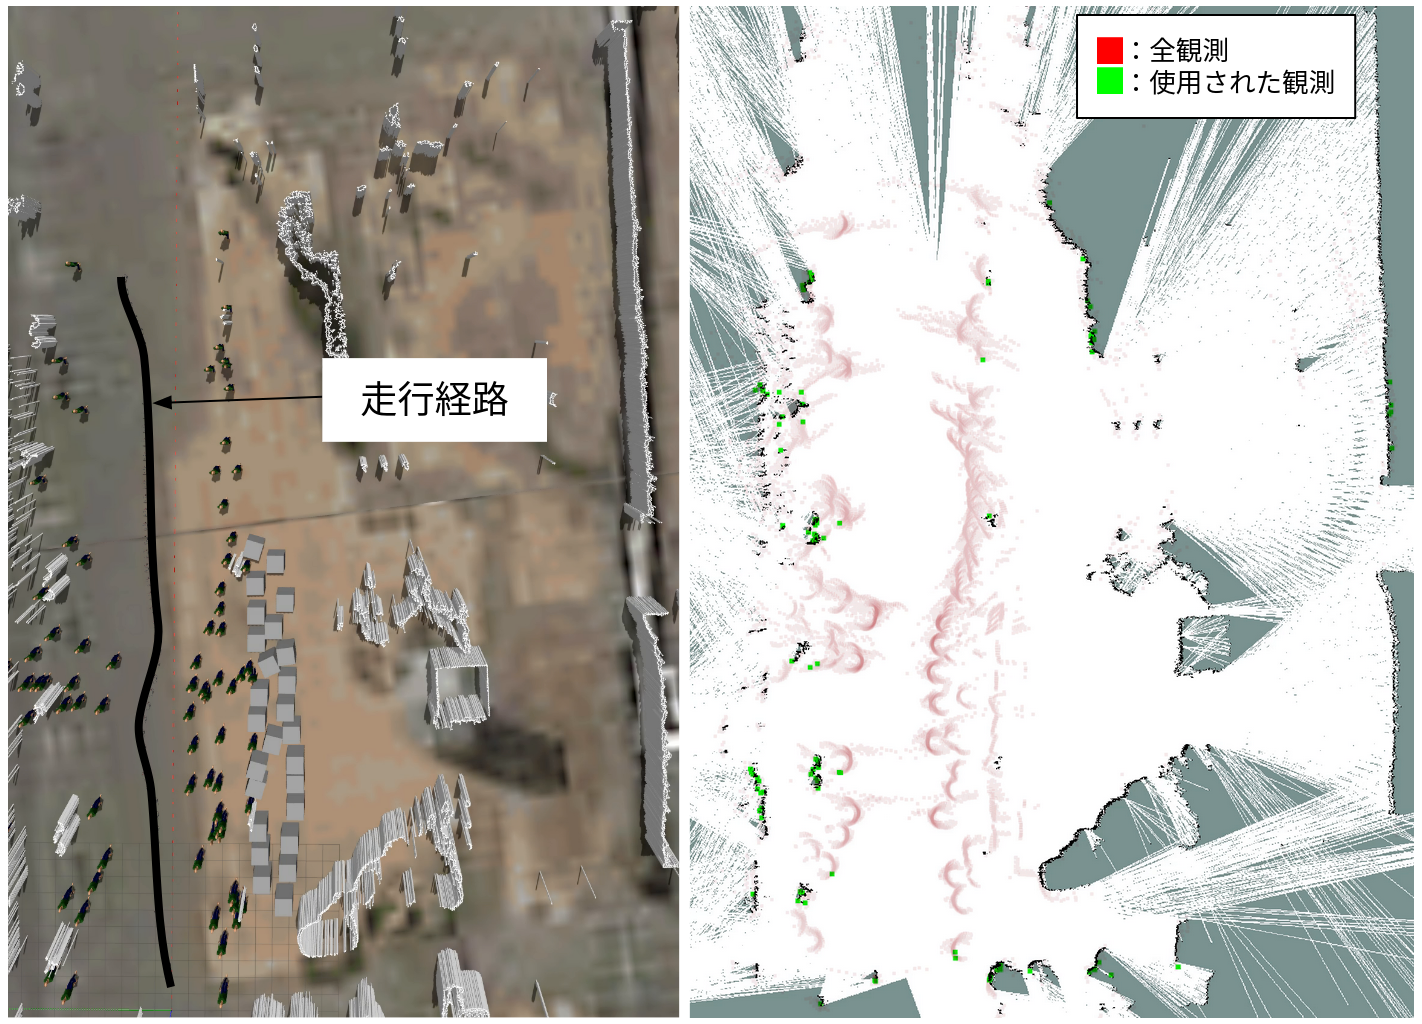
\includegraphics[width=0.8\linewidth]{fig/particle_1000_observation_1_mcl.png}
   \vspace*{-4mm}
   \caption{Navigation from start to finish (left) and visualization of observations used in the observation update (right)}
   \label{fig:スタートからゴールまでナビゲーション}
\end{figure}

% \subsection{実装による計算時間の増減}

% 自己位置の推定誤差が小さかった4つの条件
% \textcircled{\scriptsize 2}\textcircled{\scriptsize 5}\noindent
% \textcircled{\scriptsize 6}\textcircled{\scriptsize 10}\noindent
% と、元のMCLと同じ条件である
% \textcircled{\scriptsize 3}\noindent
% において、観測更新の計算時間を計測した。
% 計測した時間の結果を表\ref{table:観測更新の計算時間}に示す。
% 条件
% \textcircled{\scriptsize 3}\textcircled{\scriptsize 2}\noindent
% の結果を比較すると、観測範囲を狭めた場合、
% 実装以前よりも計算時間が減少することがわかった。
% また、パーティクルを3000から10000個に増やした時の計算時間は
% \textcircled{\scriptsize 2}\textcircled{\scriptsize 6}\noindent
% 相関して、3倍に増加していることがわかる。

% \begin{table}[htbp]
%   \caption{Computation time for observation updates under each particle condition}
%   \label{table:観測更新の計算時間}
%   \centering
%   \begin{tabular}{|c|r|r|r|} \hline
%   条件番号 & 平均[ms] & 標準偏差[ms]  \\ \hline \hline
%   \textcircled{\scriptsize 3} & 8.6 & 2.0   \\ \hline
%   \textcircled{\scriptsize 2} & 8.0 & 1.0   \\ \hline
%   \textcircled{\scriptsize 6} & 25.9 & 1.71 \\ \hline
%   \textcircled{\scriptsize 10} & 28.1 & 1.9  \\ \hline
%   \end{tabular}
% \end{table}


\section{結言}%===========================

本稿では、各パーティクルごとにランダムな観測範囲を
付与した場合のMCLの性能や良さそうな条件を実験により求めた。
実験結果からは、各パーティクルごとにランダムな観測範囲を
付与した場合のMCLは、パーティクルに付与する観測範囲が狭いほど、
未知障害物が多く存在する環境下での、自己位置の推定性能が高いことがわかった。
また、完走率が低くなってしまっているが、パーティクルに付与する観測範囲が狭い条件で、
パーティクルの数を増やすことで自己位置の推定誤差を小さくできる可能性があることがわかった。


\footnotesize
\begin{thebibliography}{99}

  \bibitem{gutmann2002}
  Jens-Steffen Gutmann and Dieter Fox: 
  ``An Experimental Comparison of Localization Methods Continued,''
  Proc. of the IEEE/RSJ International Conference on Intelligent Robots and Systems (IROS),pp. 454-459、2002.

  \bibitem{つくばチャレンジ}
  油田信一:“つくばチャレンジ: 市街地における移動ロボットの自律走行の公開実験 —11 年の経緯と成果—,''
  第 23 回ロボティクスシンポジア講演論文集, (2018), pp.59-66.
  
  \bibitem{富沢2012}
  冨沢 哲雄 and 村松 聡 and 平井 雅尊 and 佐藤 晶則 and 工藤 俊亮 and 末廣 尚士:
  ``グリッドマップのマッチングに基づく未知障害物にロバストな自己位置推定,'' 日本ロボット学会誌, 30(3):280-286, 2012.
  
  \bibitem{赤井2019}
  赤井 直紀 and モラレス ルイス 洋一 and 平山 高嗣 and 村瀬 洋:
  ``幾何地図上での観測物体の有無を考慮した自己位置推定,'' 計測自動制御学会論文集, 55(11):745-753, 2019.
  
  \bibitem{ROS}
	Morgan Quigley {\it et al.}: ``ROS: an open-source Robot Operating System,'' 
  Open-Source Software workshop of the International Conference on Robotics and Automation、2009. 

\end{thebibliography}

\normalsize
\end{document}
